\chapter{Implementacja}

W tej części pracy zostanie szczegółowo omówiona implementacja systemu eBOKa „Harmony Home Net”, która stanowi kluczowy etap realizacji projektu. Proces implementacji polega na przełożeniu założeń architektonicznych, wymagań funkcjonalnych oraz niefunkcjonalnych na działający kod, a także integracji poszczególnych komponentów systemu w spójną całość.

Wdrożenie to obejmuje zarówno warstwę frontendową, odpowiadającą za interakcje użytkowników, jak i backend, zajmujący się logiką biznesową i zarządzaniem danymi. Kluczowym elementem implementacji jest również integracja z bazą danych PostgreSQL uruchomioną w środowisku Docker, co zapewnia elastyczność, łatwość zarządzania i skalowalność.

W trakcie implementacji szczególny nacisk zostanie położony na wybór odpowiednich narzędzi i technologii, takich jak Next.js dla frontendu oraz Spring Boot dla backendu, a także Docker dla konteneryzacji systemu. Zostaną także omówione aspekty związane z optymalizacją kodu, testowaniem aplikacji oraz monitorowaniem jej działania.

Rozdział ten rozpoczyna się od przedstawienia zastosowanej \textbf{architektury warstwowej}~\cite{n_tier_wiki}, która jest podstawą projektowanego systemu. Szczegółowo opisane zostaną wszystkie warstwy – prezentacji, logiki biznesowej oraz dostępu do danych – z uwzględnieniem ich ról oraz sposobu implementacji. Następnie przejdziemy do analizy projektu \textbf{bazy danych}, gdzie omówione zostaną podejścia Database First i Code First, wraz z uzasadnieniem wyboru pierwszego z nich. Szczegółowo przedstawiona zostanie struktura bazy danych oraz sposób jej integracji z aplikacją.

Kolejnym krokiem jest omówienie kluczowych elementów zaimplementowanych w systemie. Rozpoczniemy od \textbf{bezpieczeństwa}, w tym mechanizmów autoryzacji i uwierzytelniania zrealizowanych przy użyciu Spring Security. Następnie zostanie opisane \textbf{zarządzanie mieszkańcami} jako centralny element systemu, a także inne istotne funkcje, takie jak zarządzanie mieszkaniami, zgłoszeniami technicznymi, płatnościami i powiadomieniami.

Celem tej części pracy jest nie tylko opisanie kroków wdrożenia, ale również ukazanie, w jaki sposób zaimplementowane rozwiązania odpowiadają na postawione wymagania funkcjonalne i niefunkcjonalne. Rozdział kończy się krótkim podsumowaniem, które ocenia, jak wdrożone funkcjonalności wpisują się w założenia projektu oraz wskazuje potencjalne kierunki dalszego rozwoju aplikacji.


\section{Architektura warstwowa}

Architektura warstwowa jest jednym z najbardziej rozpowszechnionych wzorców projektowych w inżynierii oprogramowania. Polega na podziale aplikacji na logiczne warstwy, z których każda pełni określoną funkcję. Taki podział ułatwia zarządzanie kodem, jego rozwój oraz utrzymanie. W typowej architekturze warstwowej wyróżnia się cztery kluczowe warstwy: warstwę prezentacji, logiki biznesowej, dostępu do danych oraz warstwę danych~\cite{n_tier_baeldung, n_tier_medium}. Ich ogólny schemat przedstawiono na rysunku \ref{fig:n_tier_arch}. Poszczególne elementy schematu oznaczono literami (a, b, c, d), co pozwala na ich jednoznaczną identyfikację w dalszym opisie.

\begin{figure}[ht]
    \centering
    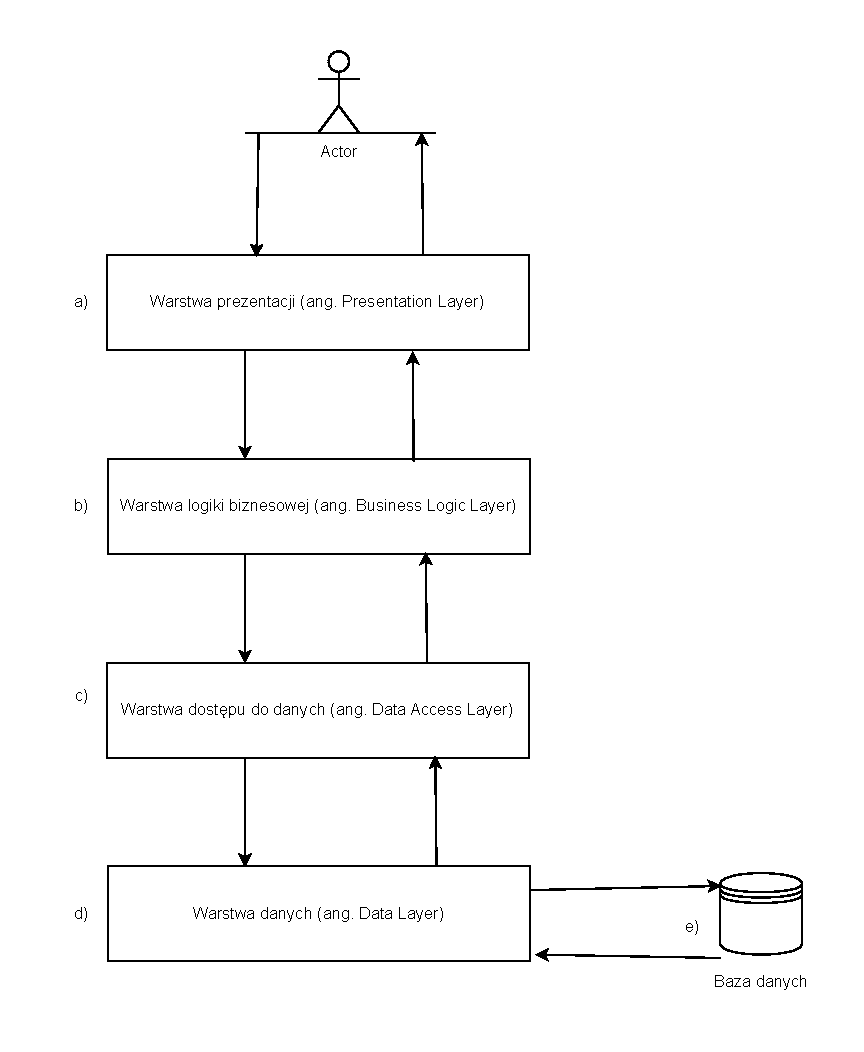
\includegraphics[width=.9\linewidth]{rys03/diagram_architektury_warstwowej}
    \caption{Ogólny schemat architektury warstwowej}
    \label{fig:n_tier_arch}
\end{figure}

\subsection{Warstwa prezentacji (ang. Presentation Layer)}
Warstwa prezentacji odpowiada za interakcję użytkownika z aplikacją, będąc głównym punktem styku użytkownika z systemem. Na tym poziomie użytkownik wprowadza dane wejściowe, a system zwraca wyniki w formie czytelnej i zrozumiałej. Głównym zadaniem warstwy prezentacji jest renderowanie interfejsu użytkownika oraz obsługa zdarzeń takich jak kliknięcia czy przesunięcia. Odpowiada również za wstępną walidację danych wejściowych, na przykład sprawdzanie, czy wprowadzony adres e-mail ma poprawny format. Przetworzone dane są następnie przekazywane do warstwy logiki biznesowej, gdzie są dalej analizowane i przetwarzane.

Na schemacie (rysunek \ref{fig:n_tier_arch}) warstwa prezentacji jest oznaczona jako element ,,\textbf{a)}''. W systemie ,,Harmony Home Net,, została zrealizowana za pomocą frameworka Next.js w języku TypeScript. Odpowiada ona za wyświetlanie interfejsu użytkownika, w tym panelu mieszkańca, gdzie użytkownicy mogą przeglądać zgłoszenia techniczne, dokonywać płatności oraz uczestniczyć w głosowaniach. Użycie Next.js umożliwia renderowanie po stronie serwera, co poprawia wydajność aplikacji oraz jej pozycjonowanie w wyszukiwarkach (SEO). Dzięki komponentom wielokrotnego użytku interfejs użytkownika jest spójny wizualnie i funkcjonalnie. 

\subsection{Warstwa logiki biznesowej (ang. Business Logic Layer)}

Warstwa logiki biznesowej pełni kluczową rolę w przetwarzaniu danych wejściowych i realizacji reguł biznesowych. Na tym poziomie dane są analizowane i przetwarzane zgodnie z zasadami określonymi przez specyfikę aplikacji. Główne zadania tej warstwy obejmują koordynację przepływu danych między innymi warstwami oraz obsługę wyjątków, które mogą wystąpić w wyniku błędów na wcześniejszych etapach przetwarzania.

Na schemacie (rysunek \ref{fig:n_tier_arch}) warstwa logiki biznesowej jest oznaczona jako element ,,\textbf{b)}''. W systemie ,,Harmony Home Net,, warstwa ta, oparta na Spring Boot, realizuje procesy biznesowe takie jak autoryzacja użytkowników przy użyciu OAuth 2.0, zarządzanie zgłoszeniami technicznymi oraz integracja z systemami płatności. Warstwa ta komunikuje się z frontendem poprzez REST API, co zapewnia efektywne przetwarzanie żądań i odpowiedzi. Dodatkowo technologia Spring Boot umożliwia implementację skalowalnych i bezpiecznych rozwiązań, co jest kluczowe w przypadku obsługi dużej liczby użytkowników.

\subsection{Warstwa dostępu do danych (ang. Data Access Layer)}

Warstwa dostępu do danych odpowiada za komunikację między logiką biznesową a fizycznym przechowywaniem danych. Jej główną funkcją jest wykonywanie operacji takich jak zapisywanie, odczytywanie, aktualizowanie i usuwanie danych w sposób zoptymalizowany i bezpieczny. Często korzysta się z bibliotek ORM, takich jak Hibernate lub JPA w Javie, które ułatwiają mapowanie danych między bazą a obiektami aplikacji.

Na schemacie (rysunek \ref{fig:n_tier_arch}) warstwa dostępu do danych jest oznaczona jako element ,,\textbf{c)}''. W systemie ,,Harmony Home Net,, baza danych PostgreSQL została uruchomiona w środowisku Docker. Dzięki zastosowaniu JPA możliwe jest łatwe mapowanie danych między tabelami bazodanowymi a obiektami aplikacji w Javie. Taka implementacja umożliwia optymalizację zapytań i zapewnia wydajność operacji, co jest istotne w przypadku dużej ilości danych przechowywanych w systemie, takich jak zgłoszenia techniczne czy płatności mieszkańców.

\subsection{Warstwa danych (ang. Data Layer)}

Warstwa danych odpowiada za trwałe przechowywanie danych aplikacji w bazach danych. Obejmuje zarządzanie strukturą danych, ich bezpieczeństwem oraz udostępnianie ich innym warstwom w sposób wydajny i zorganizowany. W systemie ,,Harmony Home Net'' wykorzystano bazę danych PostgreSQL, która została wdrożona w kontenerze Docker. 

Na schemacie (rysunek \ref{fig:n_tier_arch}) warstwa danych jest oznaczona jako element ,,\textbf{d)}''. Dzięki zastosowaniu mapowania ORM dane w bazie są bezpośrednio odwzorowywane na obiekty w aplikacji, co pozwala na wygodniejsze operacje na danych. Mechanizm ORM umożliwia wykonywanie zapytań SQL w sposób abstrakcyjny i bardziej czytelny, co upraszcza implementację i zmniejsza ryzyko błędów.

\subsection{Zalety architektury warstwowej}

Podział na warstwy przynosi wiele korzyści:
\begin{itemize}
    \item \textbf{Modularność} -- niezależność warstw ułatwia rozwój i utrzymanie systemu.
    \item \textbf{Reużywalność} -- komponenty poszczególnych warstw mogą być łatwo wykorzystane w innych projektach.
    \item \textbf{Skalowalność} -- każda warstwa może być skalowana oddzielnie, co zwiększa elastyczność aplikacji.
    \item \textbf{Czytelność kodu} -- wyraźny podział odpowiedzialności sprawia, że kod jest bardziej przejrzysty.
    \item \textbf{Testowalność} -- warstwy mogą być testowane oddzielnie, co ułatwia identyfikację błędów.
\end{itemize}

\subsection{Wady architektury warstwowej}

\begin{itemize}
    \item \textbf{Potencjalny narzut} -- dodatkowe poziomy abstrakcji mogą obniżyć wydajność systemu.
    \item \textbf{Złożoność implementacji} -- wymaga dokładnego zaplanowania, aby uniknąć nadmiernego zagnieżdżania warstw.
    \item \textbf{Brak elastyczności} -- w pewnych scenariuszach może być trudno dostosować architekturę do nietypowych wymagań.
\end{itemize}

\noindent Podsumowując, zastosowanie architektury warstwowej w systemie „Harmony Home Net” umożliwiło jego modularność, skalowalność oraz łatwość utrzymania, spełniając wymagania zarówno użytkowników końcowych, jak i administratorów.

\section{Struktura bazy danych}

Projektowanie bazy danych to jeden z kluczowych etapów tworzenia systemów informatycznych. W kontekście systemu ,,Harmony Home Net'' zdecydowano się na podejście \emph{Database First}, które polega na zaprojektowaniu struktury bazy danych przed rozpoczęciem implementacji kodu aplikacji. Jest to jedno z dwóch popularnych podejść do projektowania baz danych w aplikacjach, obok \emph{Code First}~\cite{DB_FIRST_VS_CODE_FIRST_1,DB_FIRST_VS_CODE_FIRST_2}.

\subsection{Porównanie podejść Database First i Code First}

Podejście \emph{Code First} zakłada najpierw zaprojektowanie modelu danych w kodzie aplikacji, a następnie generowanie schematu bazy danych na podstawie tego modelu~\cite{CODE_FIRST}. To rozwiązanie charakteryzuje się dużą elastycznością, co pozwala na dynamiczne zmiany w strukturze danych podczas rozwoju aplikacji. Jest ono szczególnie przydatne w projektach, gdzie schemat bazy danych może często ewoluować w odpowiedzi na zmieniające się wymagania biznesowe. Jednakże, z uwagi na brak wstępnego schematu, podejście \emph{Code First} może być trudniejsze do utrzymania w dużych projektach, w których schemat danych jest złożony i wymaga precyzyjnej kontroli.

Z kolei podejście \emph{Database First} polega na wcześniejszym zaprojektowaniu schematu bazy danych, a następnie wygenerowaniu modelu aplikacji na jego podstawie. Jest to podejście bardziej tradycyjne, które umożliwia dokładne zdefiniowanie struktury danych jeszcze przed rozpoczęciem kodowania aplikacji~\cite{DB_FIRST}. Taka metodologia daje większą przewidywalność i precyzję, co jest istotne w systemach o wysokim stopniu zależności od integralności danych. Dodatkowo, podejście to pozwala na pełne wykorzystanie możliwości narzędzi ORM, takich jak JPA, ponieważ bazuje na uprzednio zaprojektowanym schemacie.

\subsection{Wyboru podejścia Database First w systemie ,,Harmony Home Net''}

W systemie \textbf{Harmony Home Net} zdecydowano się na podejście \emph{Database First} z kilku kluczowych powodów:

\begin{itemize}
    \item \textbf{Centralna rola bazy danych} -- baza danych pełni kluczową funkcję w systemie, przechowując informacje o użytkownikach, lokalach, zgłoszeniach technicznych oraz płatnościach. Precyzyjne zaprojektowanie jej struktury na etapie początkowym pozwoliło na lepsze zrozumienie relacji między danymi i ich hierarchii.
    \item \textbf{Integracja z narzędziami ORM} -- dzięki wykorzystaniu podejścia \emph{Database First}, istniejące narzędzia ORM, takie jak JPA (Java Persistence API), mogły zostać bezproblemowo dostosowane do uprzednio przygotowanego schematu bazy danych, co uprościło implementację i zmniejszyło ryzyko błędów.
    \item \textbf{Zgodność z wymaganiami aplikacji} -- rozpoczęcie od projektowania bazy danych zapewniło pełną zgodność struktury danych z wymaganiami funkcjonalnymi i niefunkcjonalnymi systemu. Umożliwiło to również identyfikację potencjalnych problemów na wczesnym etapie prac.
    \item \textbf{Bezpieczeństwo i integralność danych} -- projektując bazę danych jako pierwszą, można było od razu uwzględnić mechanizmy zabezpieczeń, takie jak klucze główne, obce oraz indeksy. To podejście zminimalizowało ryzyko wystąpienia niespójności danych w trakcie działania systemu.
\end{itemize}

\subsection{Opis struktury bazy danych w systemie ,,Harmony Home Net''}

Struktura bazy danych w systemie \textbf{Harmony Home Net} została zaprojektowana z uwzględnieniem wymagań funkcjonalnych i niefunkcjonalnych aplikacji. Schemat bazy danych podzielono na warstwę konceptualną (rysunek \ref{fig:ebok_db_concept}) oraz fizyczną (rysunek \ref{fig:ebok_db_physical}), co umożliwiło dokładne odwzorowanie relacji pomiędzy danymi oraz optymalizację ich przechowywania.

\begin{figure}[ht]
    \centering
    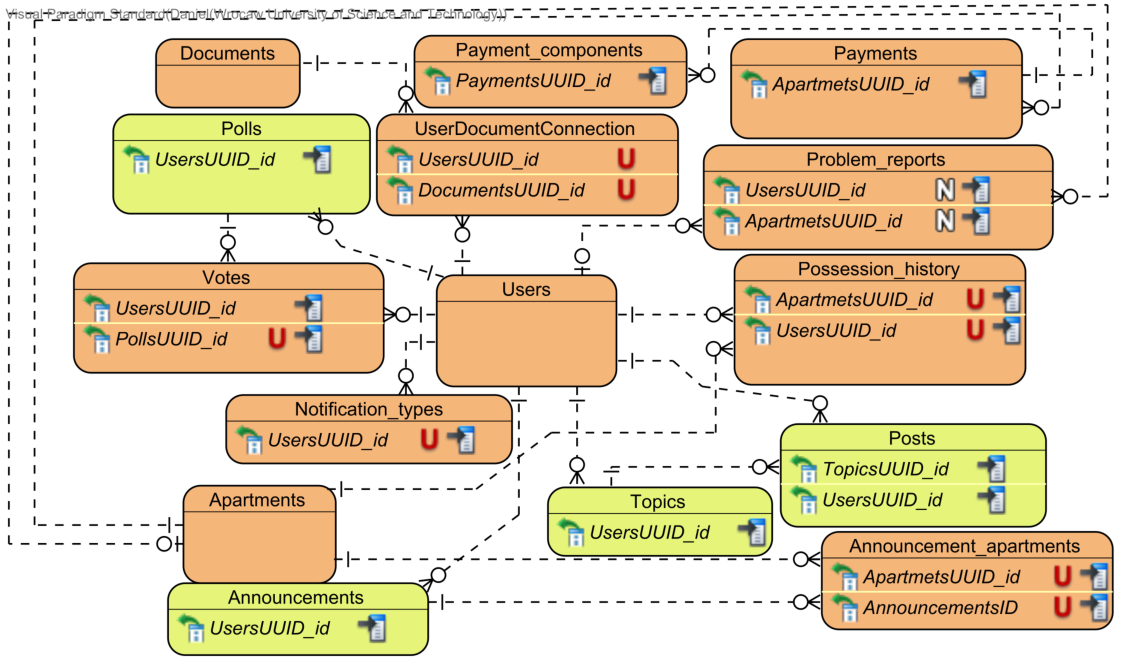
\includegraphics[width=.9\linewidth]{rys03/ebok_db_concept}
    \caption{Schemat konceptualny bazy danych systemu}
    \label{fig:ebok_db_concept}
\end{figure}

\begin{figure}[ht]
    \centering
    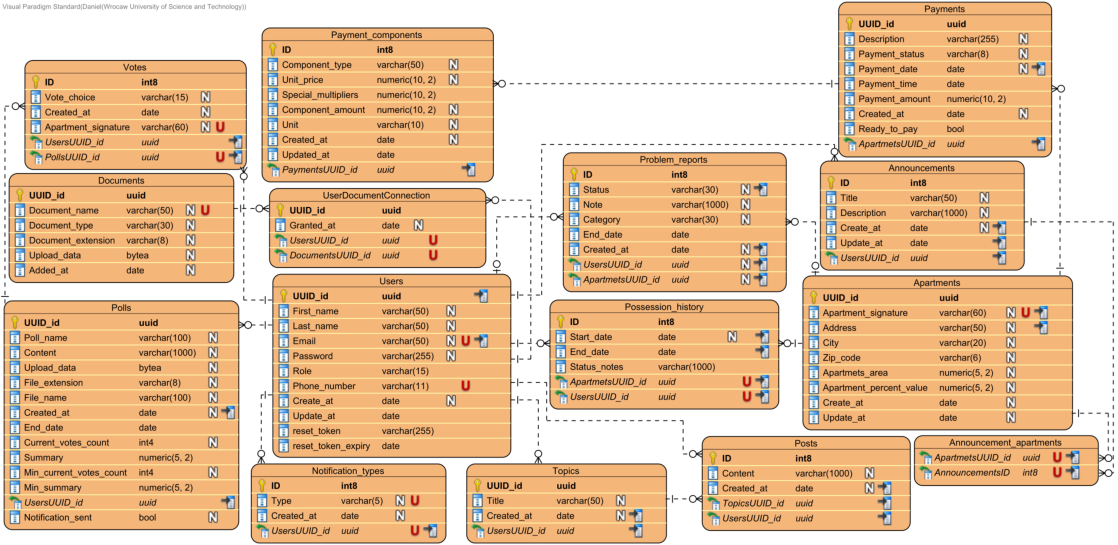
\includegraphics[width=.9\linewidth]{rys03/ebok_db_physical}
    \caption{Schemat fizyczny bazy danych systemu}
    \label{fig:ebok_db_physical}
\end{figure}

\subsubsection{Opis tabel}

Poniżej szczegółowo opisano wszystkie tabele w bazie danych:

\begin{itemize}
    \item \textbf{Tabela \texttt{Users}:}
    Przechowuje dane o użytkownikach, takie jak:
    \begin{itemize}
        \item \texttt{FirstName} i \texttt{LastName} -- imię i nazwisko użytkownika,
        \item \texttt{Email} -- unikalny adres e-mail,
        \item \texttt{Password} -- zaszyfrowane hasło,
        \item \texttt{Role} -- rola w systemie (np. właściciel, pracownik, administrator),
        \item \texttt{CreateAt} i \texttt{UpdateAt} -- daty utworzenia i ostatniej modyfikacji rekordu.
    \end{itemize}
    Klucz główny \texttt{UUID} jest wykorzystywany jako klucz obcy w wielu innych tabelach, zapewniając spójność relacji.

    \item \textbf{Tabela \texttt{Apartments}:}
    Zawiera szczegółowe dane o lokalach:
    \begin{itemize}
        \item \texttt{ApartmentSignature} -- unikalny identyfikator lokalu,
        \item \texttt{Address}, \texttt{City} i \texttt{ZipCode} -- adres lokalu,
        \item \texttt{ApartmentArea} -- powierzchnia,
        \item \texttt{ApartmentPercentValue} -- udział procentowy w nieruchomości wspólnej.
    \end{itemize}
    Powiązana z użytkownikami poprzez klucz obcy \texttt{UsersUUID}.
    
    \item \textbf{Tabela \texttt{Payments}:}
    Rejestruje dane o płatnościach:
    \begin{itemize}
        \item \texttt{Description}, \texttt{PaymentStatus}, \texttt{PaymentDate}, \texttt{PaymentAmount},
        \item \texttt{ReadyToPay} -- znacznik stanu płatności.
    \end{itemize}

    \item \textbf{Tabela \texttt{PaymentComponent}:}
    Szczegółowo opisuje składniki płatności, co pozwala na większą elastyczność w obliczaniu należności. Przechowuje informacje takie jak:
    \begin{itemize}
        \item \texttt{ComponentType} -- typ składnika płatności (np. czynsz, media, fundusz remontowy),
        \item \texttt{UnitPrice} i \texttt{ComponentAmount} -- cena jednostkowa i łączna kwota dla składnika,
        \item \texttt{SpecialMultipliers} -- specjalne mnożniki stosowane w obliczeniach (np. liczba osób, powierzchnia lokalu),
        \item \texttt{Unit} -- jednostka składnika (np. m\textsuperscript{2}, sztuki).
    \end{itemize}
    Tabela jest powiązana z tabelą \texttt{Payments} poprzez klucz obcy \texttt{PaymentsUUID}.

    \item \textbf{Tabela \texttt{ProblemReports}:}
    Zawiera zgłoszenia techniczne dotyczące lokali:
    \begin{itemize}
        \item \texttt{Status}, \texttt{Category}, \texttt{Note} -- szczegóły zgłoszenia,
        \item Klucze obce \texttt{UsersUUID} i \texttt{ApartmentsUUID}.
    \end{itemize}

    \item \textbf{Tabela \texttt{Polls} i \texttt{Votes}:}
    Obsługuje głosowania:
    \begin{itemize}
        \item Tabela \texttt{Polls} zawiera dane głosowań, a \texttt{Votes} przechowuje głosy użytkowników,
        \item Wprowadzono ograniczenie unikalności głosów w relacji \texttt{pollId} oraz \texttt{apartmentSignature}.
    \end{itemize}

    \item \textbf{Tabela \texttt{Documents} i \texttt{UserDocumentConnection}:}
    \texttt{UserDocumentConnection} pełni rolę łącznika w relacji wiele do wielu między \texttt{Users} a \texttt{Documents}. Tabela \texttt{Documents} przechowuje informacje o plikach, takie jak nazwa, typ, treść (\texttt{UploadData}) oraz data dodania.
    
    \item \textbf{Tabela \texttt{Announcements} i \texttt{AnnouncementApartment}:}
    \texttt{Announcements} przechowuje ogłoszenia, a \texttt{AnnouncementApartment} pełni rolę tabeli łącznikowej w relacji wiele do wielu między \texttt{Announcements} a \texttt{Apartments}.

    \item \textbf{Tabela \texttt{NotificationTypes}:}
    Przechowuje różne typy powiadomień i ich relacje z użytkownikami. Zdefiniowano ograniczenie unikalności, które uniemożliwia przypisanie tego samego typu powiadomienia temu samemu użytkownikowi wielokrotnie.

    \item \textbf{Tabela \texttt{PossessionHistory}:}
    Rejestruje historię przypisania użytkowników do lokali:
    \begin{itemize}
        \item \texttt{StartDate} i \texttt{EndDate} -- okres użytkowania lokalu,
        \item Klucze obce \texttt{ApartmentsUUID} i \texttt{UsersUUID}.
        \item Zastosowano ograniczenie unikalności relacji między \texttt{userId} a \texttt{apartmentId}.
    \end{itemize}
\end{itemize}

\subsubsection{Podział tabel na pakiety}

W implementacji kodu wszystkie tabele zostały podzielone na dwa logiczne pakiety:
\begin{itemize}
    \item \textbf{Pakiet \texttt{sideTables}:} Obejmuje tabele pomocnicze, które pełnią rolę łączników w relacjach wiele do wielu. Należą do niego:
    \begin{itemize}
        \item \texttt{UserDocumentConnection},
        \item \texttt{PossessionHistory},
        \item \texttt{AnnouncementApartment}.
    \end{itemize}

    \item \textbf{Pakiet \texttt{mainTables}:} Obejmuje główne tabele przechowujące kluczowe dane systemu, takie jak:
    \begin{itemize}
        \item \texttt{Users},
        \item \texttt{Apartments},
        \item \texttt{Payments},
        \item \texttt{PaymentComponent},
        \item \texttt{ProblemReports},
        \item \texttt{Polls},
        \item \texttt{Votes},
        \item \texttt{Documents},
        \item \texttt{Announcements},
        \item \texttt{NotificationTypes}.
    \end{itemize}
\end{itemize}

Podział tabel na dwa pakiety zapewnia przejrzystość struktury kodu, łatwość zarządzania relacjami między encjami oraz ułatwia przyszłą rozbudowę systemu.


\subsection{Relacje i integralność danych}

Relacje między tabelami zostały szczegółowo odwzorowane za pomocą kluczy głównych i obcych, co umożliwia utrzymanie integralności danych oraz łatwe zarządzanie połączeniami między różnymi elementami bazy. Na przykład, tabela \texttt{Problem\_reports} zawiera klucze obce do tabel \texttt{Users} i \texttt{Apartments}, co pozwala na przypisanie zgłoszeń technicznych zarówno do konkretnego użytkownika, jak i lokalu. Analogicznie, tabela \texttt{Payments} jest powiązana z tabelą \texttt{Apartments}, co zapewnia pełną kontrolę nad płatnościami przypisanymi do danych lokali.

\subsection{Mechanizmy optymalizacyjne}

W celu poprawy wydajności bazy danych zastosowano następujące mechanizmy:
\begin{itemize}
    \item \textbf{Indeksy} -- kluczowe kolumny, takie jak \texttt{UUID}, zostały zaindeksowane w celu przyspieszenia operacji wyszukiwania i sortowania.
    \item \textbf{Mapowanie ORM} -- baza danych została zintegrowana z aplikacją za pomocą narzędzia JPA (Java Persistence API), co umożliwia bezpośrednie mapowanie tabel na obiekty w kodzie aplikacji. Dzięki temu operacje CRUD (Create, Read, Update, Delete) mogą być realizowane w sposób wygodny i abstrakcyjny, bez konieczności pisania zapytań SQL.
    \item \textbf{Konteneryzacja} -- PostgreSQL działa w środowisku Docker, co zapewnia łatwość zarządzania i możliwość skalowania systemu w zależności od obciążenia.
		\item \textbf{Ograniczenia unikalności (ang. Unique Constraint)} -- w tabelach takich jak \texttt{Votes}, \texttt{PossessionHistory}, \texttt{NotificationTypes}, oraz \texttt{AnnouncementApartment} zastosowano ograniczenia unikalności (\texttt{UniqueConstraints}), co zapobiega wprowadzaniu niepożądanych duplikatów w relacjach wiele do wielu.
\end{itemize}

\subsection{Podsumowanie}

Struktura bazy danych systemu \textbf{Harmony Home Net} została zaprojektowana w sposób umożliwiający jej skalowalność, wydajność oraz łatwość integracji z innymi komponentami aplikacji. Podejście \emph{Database First} okazało się optymalnym wyborem, zapewniając precyzyjne odwzorowanie wymagań biznesowych i technicznych systemu. Schematy konceptualny (rysunek \ref{fig:ebok_db_concept}) i fizyczny (rysunek \ref{fig:ebok_db_physical}) ilustrują relacje pomiędzy tabelami, które stanowią podstawę spójnego i efektywnego zarządzania danymi.




\section{Bezpieczeństwo, uwierzytelnianie i autoryzacja w aplikacji}

\section{Zarządzie użytkownikami}

\section{Zarządzie mieszkaniami}

\section{Zarządzie dokumentami}

\section{Zarządzie zgłoszeniami problemów}

\section{Zarządzie ogłoszeniami}

\section{Zarządzie forum dla wspólnoty}

\section{Zarządzie płatnościami}

\section{Zarządzie głosowaniami}

\section{Systemy zewnętrzne}



